\documentclass[spanish,12pt,letterpapper]{article}
\usepackage{babel}
\usepackage[utf8]{inputenc}
\usepackage{graphicx}
\usepackage{hyperref}
\begin{document}
	\begin{titlepage}
		\begin{center}
			
\includegraphics[width=0.6\textwidth]{../logoUnADM}~\\[1cm] 
			\textsc{Universidad Abierta y a Distancia de M\'exico}\\[0.8cm]
			\textsc{Desarrollo de Software}\\[1.8cm]
			
			\textbf{ \Large Actividad 2. Programación de un arbol}\\[3cm]
			
			Diego Antonio Plascencia Lara\\ ES1421004131 \\[0.4cm]
			Facilitador(a): Alejandro Francisco Marquez Fuentes\\
			Asignatura: Estructura de datos\\
			Grupo: DS-DEDA-1502S-B1-002 \\
			Unidad: III \\
			
			\vfill M\'exico D.F\\{\today}
			
		\end{center}
	\end{titlepage}
	
	\textbf{1. Resuelve de forma muy sencilla con estos pasos y crea la imagen del árbol que a continuación se describe :\\}
	a) Se toma el dato a ingresar X\\
	b) Partiendo de la raíz preguntamos: Nodo == null ( o no existe ) ?\\
	c) En caso afirmativo X pasa a ocupar el lugar del nodo y ya hemos ingresado nuestro primer dato.\\
	d) En caso negativo preguntamos: X < Nodo\\
	e) En caso de ser menor pasamos al Nodo de la IZQUIERDA del que acabamos de preguntar y repetimos desde el paso 2 partiendo del Nodo al que acabamos de visitar\\
	f) En caso de ser mayor pasamos al Nodo de la DERECHA y tal cual hicimos con el caso anterior repetimos desde el paso 2 partiendo de este nuevo Nodo.\\
	
	En este caso se trata de un árbol binario, y un ejemplo de un árbol binario es el siguiente, utilizando en este caso números como x:\\
	
	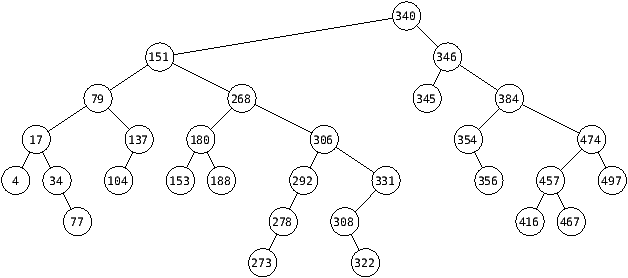
\includegraphics[width=1\textwidth]{./arbolbinario}~\\[1cm]
	\pagebreak
	
	
	\textbf{2. A partir de la información investigada, describe un ejemplo de cómo se aplica en un caso cotidiano junto con su imagen de arbol\\}
	Un ejemplo practico seria la implementación de un sistema en donde se tienen que almacenar y ordenar fechas ligados a eventos, primero el nodo raíz se establecería como la fecha 0, después al querer ordenar y almacenar una serie de eventos, se entraría la fecha y por el algoritmo del árbol binario se ordenaría según la fecha, para posteriormente poder buscar el evento por la fecha.\\
	
	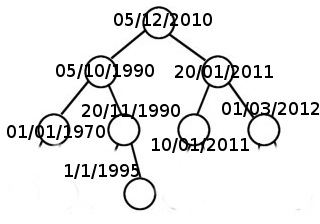
\includegraphics[width=1\textwidth]{./abinariomod}~\\[1cm]
	\pagebreak
		
	\textbf{3. Finalmente, redacta una breve conclusión en torno al tema\\}
	Los arboles binarios son importantes para el almacenamiento de datos de una forma mas eficiente para después poder realizar una búsqueda, el algoritmo del árbol binario implícitamente lleva un orden, por esto hace eficiente su búsqueda.\\
	
	Es importante aprender a implementarlos para usarlos en sistemas que se requieran almacenar y buscar gran cantidad de datos.
	
	
	\pagebreak
	\begin{thebibliography}{9}
		\bibitem{Goodrich} Goodrich, M. y Tamassia, R. (2010).
		\emph{Estructura de datos y algoritmos en Java}. México: CECSA.
		
		\bibitem{WikiWArbol} Wikipedia. 
		\emph{Árbol (informática)}.  {[} Fecha de consulta: \today {]}. Disponible en: \textless https://es.wikipedia.org/wiki/\%C3\%81rbol\_(inform\%C3\%A1tica) \textgreater
		
		\bibitem{WikiWArbol} Wikipedia. 
		\emph{Árbol binario}.  {[} Fecha de consulta: \today {]}. Disponible en: \textless https://es.wikipedia.org/wiki/\%C3\%81rbol\_binario \textgreater

	\end{thebibliography}
	
\end{document}